\section{Suggesting Changes In View(s Types)}
\label{sec:Suggestion}

Figure \ref{fig:Suggestion} depicts a \metamodel that capture the
required elements for helping methodologists improve their designs.
On the following, we assume that a methodologist is working on a \metamodel
under evolution \textsf{MM}, that is linked to a family $\mathsf{VT}$ of viewtypes
(i.e. \mathsf{VT} = $(\mathsf{VT}_i)_{i\in [1..n]}$). Note that in the discussion above, when we discuss
\textsf{MM}'s (meta-)elements, we consider \textsf{MM} as a \emph{model}
conforming to a particular meta-\metamodel (such as \textsc{Mof} \cite{TR:OMG-MOF:2016}):
we therefore discuss changes on \textsf{MM}'s packages, classes (e.g. 
\textsf{FSM} or \textsf{State} in our example) and their structural features
(such as the attribute \textsf{name} or the reference \textsf{src}).

A \textsf{Suggestion} is the core element of our approach, and contains three 
parts: a \textsf{Change}, some \textsf{Relation}s, and a list of 
\textsf{Recommendation}s. 
%
As detailed in Figure \ref{fig:Change}, a \textsf{Change} captures the nature of
alterations operated on \textsf{MM}'s meta-elements. 
A \textsf{Relation} provides tracebility links between \textsf{MM} and \textsf{VT}:
for each meta-element in \textsf{MM} subject to a \textsf{Change}, a \textsf{Relation}
identifies which meta-elements in \textsf{VT} may be affected. 
Finally, a \textsf{Recommendation} details possible actions a methodologist may 
perform to realign \textsf{VT} after the \textsf{Change}. 
Note that a \textsf{Suggestion} may 
associate \emph{no} \textsf{Recommendation}s, in case a \textsf{Change} has no
impact on \viewtypes; or \emph{several} \textsf{Recommendation}s for the same 
\textsf{Change}, depending on the complexity of the \textsf{Change}, and how 
many \viewtypes are concerned by the \textsf{Change}.

The rest of this Section details each part in a \textsf{Suggestion}; a summary
is presented in Table \ref{tab:suggestions}.

\subsection{Change}
\label{sec:Suggestion:Change}

\begin{figure}[t]
    \centering
    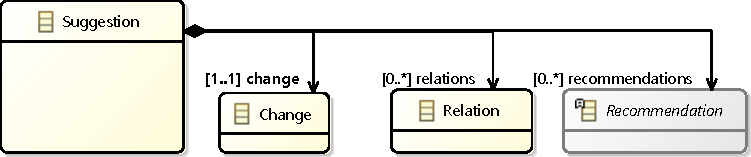
\includegraphics[width=\columnwidth]{images/Suggestion.pdf}
    \caption{A \textsf{Suggestion} holds for a single \textsf{Change} linked to 
		elements in a View Type through \textsf{Relation}s, and consists of a set of \textsf{Recommendation}s.}
    \label{fig:Suggestion}
\end{figure}

A \textsf{Change} refers to an \textsf{Operator} that may be parameterised with 
extra data, and contains contextual information (in \textsf{ApplicationPattern}). 
Change \textsf{Operator}s may target \emph{any} instanciable metamodel element, 
thus referring to the class \textsf{NamedElement} in \textsc{Mof}. Note that we 
will distinguish between \emph{primitive} and \emph{complex} \textsf{Operator}s,
depending on the number of such \metamodel elements an \textsf{Operator} acts on.

Since \viewtypes are structurally \metamodels, we reviewed the literature to
identify relevant change \textsf{Operator}s. The change catalogue proposed by 
\cite{herrmannsdoerfer_extensive_2011} presents 27 \emph{primitive}, and 34
\emph{complex} operators. We integrated all primitive, and 7 complex operators
in our work, which were selected because they constitute 72\% of all complex
changes appearing in a large case study (cf. \cite{khelladi_detecting_2015}). 

\textsf{Operator}s are enriched with a \emph{severity}: \emph{Major}
(abbreviated as \textsf{M}), \emph{miNor} (\textsf{N}) and \emph{Ignore} 
(\textsf{I}). 
When applied to a \metamodel, the \textsf{Operator}s in \textsf{I} have no effect
on the corresponding \viewtypes; \textsf{Operator}s that can break the relationship
between \textsf{MM }and its \viewtypes are categorised as \textsf{M}; the rest of the
\textsf{Operator}s are \textsf{N}, since they are not breaking and can enrich 
the \viewtypes with additional information.

\begin{figure}[t]
    \centering
    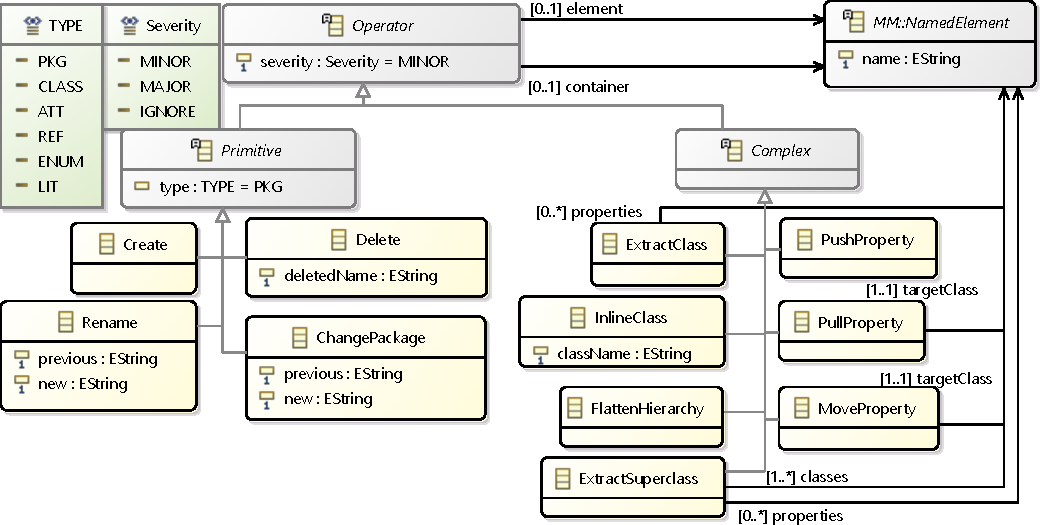
\includegraphics[width=\columnwidth]{Change.pdf}
    \caption{Possible \textsf{Operator}s for \metamodel evolution.}
    \label{fig:Change}
\end{figure}

The evolution steps of Figure \ref{fig:FSM} make use of different \textsf{Operator}s.
\begin{itemize}
	\item In Step 1 (depicted from Figure \ref{fig:FSM:Init} to \ref{fig:FSM:Relevant}),
	the following sequence of \textsf{Operator}s is applied:
	$$\langle \mathsf{PushProperty} \cdot \mathsf{Rename} \cdot \mathsf{Rename} \rangle$$
	First, \textsf{PushProperty} pushes down $\mathsf{Named} \squaredots \mathsf{name}$
	(i.e. pushes down the \textsf{element} \textsf{name} in the \textsf{container}
	\textsf{Named})
	into each subclass (namely, \textsf{FSM}, \textsf{State} and \textsf{Transition});
	then \textsf{Rename} is applied to the \textsf{element} \textsf{name}, 
	located respectively in \textsf{container}s $\mathsf{FSM}$ and 
	$\mathsf{Transition}$, thus obtaining the result of Figure \ref{fig:FSM:Relevant}.
	
	\item Step 2 only consists of the following \textsf{Operator}s sequence:
	$$\langle \mathsf{Create} \cdot \mathsf{Create} \cdot \mathsf{Create} \rangle$$
	where each \textsf{Operator} adds a new Attribute \textsf{element} in 
	\textsf{container} \textsf{Transition}, ending up in the situation of
	Figure \ref{fig:FSM:Guard}.
	
	\item Step 3 requires a longer sequence of \textsf{Operator}s, since it creates
	a new class hieararchy under \textsf{Expression}. However, this sequence may
	start with the following:
	$$\langle \mathsf{Delete}^3 \cdot \mathsf{Create}^2 \cdot \ldots \rangle$$
	The three first \textsf{Delete} undo the \textsf{Create} operations of Step 2
	(thus, referring to the same \textsf{element}s and \textsf{container}); and
	the two following \textsf{Create} create the new \textsf{Expression} class
	(with the default package as a \textsf{container}) and the \textsf{guard}
	reference (with \textsf{Transition} as a \textsf{container}).
\end{itemize}
With these examples, we immediately notice that some \textsf{Operator}s
in a \textsf{Change} sequence may depend on previous ones (e.g. \textsf{Rename}
in Step 1 should only be performed after \textsf{PushProperty}); while others
may freely commute (e.g. the \textsf{Create} in Step 2 may be performed in any 
order).
\subsection{Relation}
\label{sec:Suggestion:Relation}

The \textsf{Relation} part provides traceability links between \textsf{MM}
all the corresponding \textsf{changed} and \textsf{impacted} elements.
% elements that are \textsf{changed}, and all \viewtype elements that are 
% \textsf{impacted} by that change. 
One \textsf{MM} element change
may impact several elements in the same \viewtype, but may also potentially
impact several \viewtypes. We only require so-called \emph{links}; however richer
data structures for traceability may be used \cite{Batot-Cabot-Gerard:2021}.

The way these traceability links are computed are left as implementation
details, and may happen in two ways: \emph{on-the-fly} whenever an \textsf{MM} element is evolved; and \emph{offline}
after a complete evolution session has terminated---either based on diffing \cite{Kehrer-Kelter-Taentzer:2011}, or using 
operation-based approaches \cite{J:Lippe-Oosterom:1992}.

\begin{figure}[t]
    \centering
    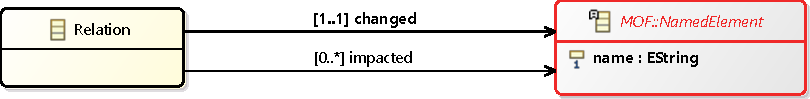
\includegraphics[width=\columnwidth]{Relation.pdf}
    \caption{\textsf{Relation}s between \textsf{MM} elements and \textsf{VT} elements.}
    \label{fig:Relation}
\end{figure}

In the \textsf{FSM} example associated to the initial \textsf{VT\_FSM} of \cref{fig:VT:VMM},
we would have, among others, the following relations (with \textsf{Link}s denoted 
as e.g.~$\mathsf{<} \mathsf{changed} ; \mathsf{impacted} \mathsf{>}$):
\begin{itemize}
	\item Since computing the \textsf{name}s in \textsf{VT\_FSM} requires access
	to $\mathsf{Named \squaredots name}$, the following \textsf{Link}s would be
	created: 
	$\mathsf{<} \mathsf{Named \squaredots name} ; \mathsf{VT\_FSM \squaredots name} \mathsf{>}$;
	$\mathsf{<} \mathsf{Named \squaredots name} ; \mathsf{State \squaredots name} \mathsf{>}$;
	$\mathsf{<} \mathsf{Named \squaredots name} ; \mathsf{Transition \squaredots name} \mathsf{>}$.

	\item Creating an instance of \textsf{State} requires to take into account
	the value of $\mathsf{State \squaredots kind}$, which would produce the following
	\textsf{Link}s: 
	$\mathsf{<} \mathsf{State \squaredots kind} ; \mathsf{State} \mathsf{>}$;
	$\mathsf{<} \mathsf{State \squaredots kind} ; \mathsf{Initial} \mathsf{>}$;
	$\mathsf{<} \mathsf{State \squaredots kind} ; \mathsf{Regular} \mathsf{>}$.
	Depending on the precision of the traceability analysis, the following may
	eventually be produced as well: 
	$\mathsf{<} \mathsf{Kind \squaredots REGULAR} ; \mathsf{Regular} \mathsf{>}$ and
	$\mathsf{<} \mathsf{Kind \squaredots INITIAL} ; \mathsf{Initial} \mathsf{>}$.
	%\LC{Again, for FINAL too?}\MA{The \textsf{Link}s are established on the initial version, \emph{\textbf{before} the evolution step. 
	%The next bullet (``After Step 2''!!!) explicitly says what you want to put here, which is a wrong place to do so.}}
	


	\item After Step 2, some \textsf{Link}s between the newly added attributes
	in $\mathsf{FSM \squaredots Transition}$ and the corresponding attributes in 
	$\mathsf{VT\_FSM \squaredots Transition}$ may be added as well. New 
	\textsf{Link}s taking into account the newly added literal in \textsf{Kind}
	would be added, similarly to the previous point.
\end{itemize}
\subsection{Recommendation}
\label{sec:Suggestion:Recommendation}

While a \textsf{Change} concerns \textsf{MM}, a \textsf{Recommendation} describes
an \textsf{Action} a methodologist may perform on \textsf{VT}. In our approach, we
issue a \textsf{Recommendation} for each \viewtype element impacted by a 
\textsf{Change}. We identified four kinds of \textsf{Action}s: a \textsf{REM}ove
\textsf{Action} indicates that a \viewtype element is no longer associated to an
\textsf{MM} element; an \textsf{ADD} suggests that a representation for a newly 
created \textsf{MM} element should be added in a \viewtype; an \textsf{UP}date
\textsf{Action} suggests to update a 


\begin{figure}[t]
    \centering
    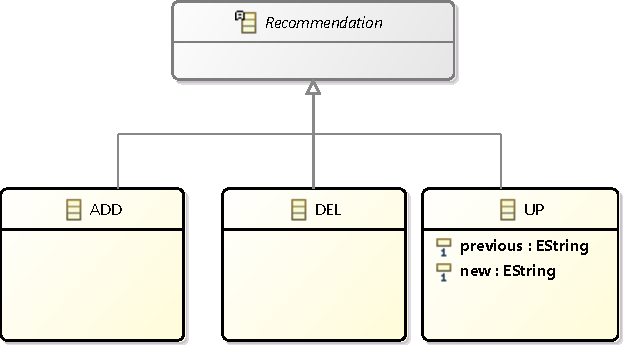
\includegraphics[width=0.8\columnwidth]{Recommendation.pdf}
    \caption{\textsf{Recommendation}s suggested after a \textsf{Change}}
    \label{fig:Change}
\end{figure}

